%------------------------------------------------------------------------------
% Template file for the submission of papers to IUCr journals in LaTeX2e
% using the iucr document class
% Copyright 1999-2013 International Union of Crystallography
% Version 1.6 (28 March 2013)
%------------------------------------------------------------------------------

\documentclass[pdf]{iucr}              % DO NOT DELETE THIS LINE
%\documentclass[preprint]{iucr} 
\usepackage{graphicx}
\usepackage{color}
\usepackage{ulem}
\usepackage{multicol}

     %-------------------------------------------------------------------------
     % Information about journal to which submitted
     %-------------------------------------------------------------------------
     \journalcode{S}              % Indicate the journal to which submitted
                                  %   A - Acta Crystallographica Section A
                                  %   B - Acta Crystallographica Section B
                                  %   C - Acta Crystallographica Section C
                                  %   D - Acta Crystallographica Section D
                                  %   E - Acta Crystallographica Section E
                                  %   F - Acta Crystallographica Section F
                                  %   J - Journal of Applied Crystallography
                                  %   M - IUCrJ
                                  %   S - Journal of Synchrotron Radiation

\begin{document}                  % DO NOT DELETE THIS LINE

     %-------------------------------------------------------------------------
     % The introductory (header) part of the paper
     %-------------------------------------------------------------------------

     % The title of the paper. Use \shorttitle to indicate an abbreviated title
     % for use in running heads (you will need to uncomment it).

\title{TomoPy: A framework for the analysis of synchrotron tomographic data}
%\shorttitle{Short Title}

     % Authors' names and addresses. Use \cauthor for the main (contact) author.
     % Use \author for all other authors. Use \aff for authors' affiliations.
     % Use lower-case letters in square brackets to link authors to their
     % affiliations; if there is only one affiliation address, remove the [a].

\cauthor{Do\v{g}a}{G\"{u}rsoy}{dgursoy@aps.anl.gov}{} 
\author{Francesco}{De Carlo}
\author{?}{?}


\aff{Advanced Photon Source, Argonne National Laboratory, 9700 S.~Cass Ave., Argonne IL 60439-4837 \country{USA}}


     % Keywords (required for Journal of Synchrotron Radiation only)
     % Use the \keyword macro for each word or phrase, e.g. 
     % \keyword{X-ray diffraction}\keyword{muscle}

\keyword{tomopgraphy}
\keyword{x-ray imaging}
\keyword{phase retrieval}

\hyphenpenalty=10000

\maketitle                        % DO NOT DELETE THIS LINE

\begin{synopsis}
Supply a synopsis of the paper for inclusion in the Table of Contents.
\end{synopsis}

\begin{abstract}
Abstract goes here.
\end{abstract}


\section{Introduction}

Analysis of large tomographic datasets at synchrotron light sources is becoming progressively more challenging  due to the increasing data acquisition rates that new technologies in X-ray sources and detectors enable. The next generation of synchrotron facilities that are currently under design or construction throughout the world will provide diffraction limited X-ray sources and is expected to boost the current data rates by several orders of magnitude and stressing the need for the development and integration of automated and efficient analysis tools more than ever. 

Several synchrotron users already collect data at different facilities to take advantage of specific instrument characteristics and specifications, but they are often left alone integrating this data with the available or home-grown software tools. However, there are often strong similarities within the same class of instruments that are not systematically utilized to build a coordinated software development platform or framework where each facility and user group can take advantage from or contribute in, ultimately saving on-site resources by sharing the computing tasks with the user community. 

Here we describe in detail an attempt to provide such a collaborative framework for the analysis of synchrotron tomographic data that has the potential to unify the effort of different facilities and beamlines performing similar tasks. The basic principles of this Python based open-source framework, called {\it TomoPy}, \cite{python_cpp}, are: easiness to collaborative development of scripts, platform and data format independent, modular,  and supporting a functional programming style that many researchers in Academia prefer. In the following sections, we will provide a brief background on the analysis of tomographic data at synchrotrons, and then shortly introduce the framework by describing the model structure together with the available methods. 


\section{Background}

When it comes to the digital storage of tomographic experimental data and the development of analysis tools at synchrotron light sources around the world, the situation is very heterogeneous (just like Babel!). As different research teams and instruments have grown at various facilities, they have often developed local data and analysis models based on the instrument hardware specificity and often drawing upon the particular preferences of a scientist writing software. 

Many tomographic analysis tools utilize licensed, and often expensive, software packages like Matlab \cite{matlab} and IDL \cite{exelis_vis}, others rely on specific, and often complex to maintain, computing infrastructure like MPI-based CPU or GPU clusters. This diversity and specializations hamper an integrated development environment and limit their long term use. On the other hand, modern chip design shows a clear trend toward integration of multiple processor cores and permits concurrency without a need for a dedicated cluster. The availability of inexpensive multi-core CPU workstations and the reduced cost of computer memory in today allow to considerably simplify the computing infrastructure required to process tomographic data \cite{rivers_spie_2012}, and make the development of single workstation tools able to perform most computing tasks at reasonable times. Besides, it allows the analysis to be performed on an off-site location, freeing on-site computational resources for other tasks. 

This transition is affecting all major synchrotron facilities where new effort is now dedicated into developing new tools that can be deployed at the facility for real time processing as well as distributed to users for off-site data processing. We believe this will pave the way for an efficient use of the existing knowledge and methods base, thereby fostering collaborations and development of novel methods.

\section{TomoPy: A python based framework}

There is no free lunch when it comes to the integration of analysis methods. For example, Matlab's or IDL's coding practice which is based on matrix and linear algebra operations that many researchers get accustomed to come with pricy licensing fees compared to open source alternatives. R, \cite{r}, as an open-source alternative, offers a wide variety of statistical data analysis tools but generally considered as having a steep learning curve and is usually hard to maintain for large projects. Low-level programming languages like C or Fortran provide the desired computational speed but lack in readability and may hinder a collaborative code development. Python with its standard library on the other hand provides a modular, readable and manageable framework that researchers can use freely or contribute easily without facing any hassles. Python is also a convenient wrapper to Python's C or Fortran application programming interface (API) which makes it easy to expose a python API to existing C, C++ or Fortran codes. Besides, the native  control software running at several synchrotron facilities, EPICS, \cite{epics}, is interfaced to Python \cite{pyepics}, allowing simultaneous data analysis and real-time feedback on the instrumentation status. These features make Python the method of choice for development framework.

TODO: Add a paragraph mentioning data format independence: Converter. Data Exchange. Output formats?

The data-driven pipeline of tomographic reconstruction allows for an easy kind of concurrency which is simply based on data parallelism. The tasks can be distributed through a queue into available processors and executed in parallel, and in many cases, there is either zero or minimal cross-talk between the distributed tasks which simplifies the implementation and exploitation of parallelism.

Digestion of synchrotron tomographic data is essentially modular in nature such that the processes can be divided into a number of independent, and in many situations serialized, steps. A natural way of segmenting these processes is to group tasks according to the similarities in transformations applied on data, that is distributing tasks into modules like pre-processing (data-to-data transformations), reconstruction (data-to-image transformations) and post-processing (image-to-image transformations). This modular pipeline design allows a degree of control for the entire process by checking the quality of individual steps taken and at the same time improves the readability of the code. The following section describes the journey of data, through multiple transformations, from acquisition to image display.


\section{Methods} 

In synchrotron tomography, the imaging sample is placed in the beam path and the x-ray intensity profiles on the detector (also called tomograms or projections) are acquired by rotating the sample during x-ray exposure. Almost all data acquisition protocols require another sets of data taken in the absence of the sample which is usually refereed to as the white-field measurements ($I_{white}$) and in the absence of X-ray exposure which is called the dark-field measurements ($I_{dark}$). The order of the multidimensional arrays is, by default, assumed as the fastest changing dimension being the last dimension, and the slowest changing dimension being the first dimension. These three sets of measurement together with the rotation angle information are the entry point of the analysis pipeline.

\subsection{Pre-processing} 

Once the data and the corresponding projection angles are imported from the HDF5 dataset, a set of default methods is available under the preprocessing module simply to prepare data for reconstruction. Generally the pipeline of functions start with the normalization which include a dark-field (offset) and gain correction of raw intensity data ($I_{raw}$) as follows:
\begin{equation}
I_{normalized}=\frac{I_{raw}-I_{dark}}{I_{white}-I_{dark}}
\end{equation}
This step is essential for almost all the time not only to compensate different sensitivities and responses in each detector pixel but also to scale the images between 0 and 1 to obtain a reliable attenuation information about the sample according to the Beer-Lambert's law. 

For most datasets, a simple normalization can not satisfactorily correct for the detection artifacts, which are usually caused by the drifts in measurements or by the non-linearity in the detector response. These imperfections appear as stripes in sinogram and transform to image domain as ring shaped artifacts. This is particularly as issue for .... (Francesco: fly scan? slow data acquisition?) data acquisition where ..... . To correct for these ring artifacts, a combined wavelet-Fourier filtering  \cite{Munch:09} is adopted. The filtering is essentially based on a set of transformations to condense the artifacts into a tiny region so that removal of them would not cause any deformations to actual features of the sample and is superior to many other filtering approaches in terms of robustness and conservation of image features (see figure).

For some samples that are either beam sensitive or have low absorption contrast like biological specimens, an in-line phase-contrast imaging (PCI) mode, which exploits Fresnel diffraction, is applied. In PCI, to retrieve phase out of the projected phase-contrast data, single-step methods are of primary importance because they allow a much faster scanning without a need to alter the detector position multiple times during data acquisition. PCI also may be utilized to separate the phase and the attenuation contrast, and ultimately to reconstruct the distribution of the real and imaginary part of the refractive index separately. Figure ? shows the phase-contrast data and the corresponding retrieved phase using the Paganin's filter.

%One of the limiting factors on reconstruction quality is that when the sample size is greater than the detector's field of view. If the ratio of the sample to detector transverse width is smaller than two, than a full projection dataset can be acquired using a 360-degrees rotation.

\subsection{Reconstruction}

The next module in the pipeline is the reconstruction module which contains functions that maps data from data space into image space. There are numerous methods suitable for this task each having both strengths and weaknesses depending on the applied data and timing constraints. As the default method, we provide Gridrec, which is a linear method that relies on discrete Fourier transforms of data similar to the filtered-backprojection method. The main difference is that it samples the Fourier domain on a regular grid before transforming back to the spatial domain. Utilizing fast Fourier transforms on regular grids outperforms other methods in terms of computational speed and is usually desired for quick reconstructions.

One of the key goals in reconstruction is to render the integration of nonlinear inversion methods possible in this framework. Nonlinear methods, also referred to as the model-based methods, try to minimize for data fidelity based on a system model, and in principle, all require an accurate forward model which mainly relies on an efficient ray-tracing implementation. To serve on this purpose, we build 2-dimensional and 3-dimensional ray-tracing algorithms that one can use to construct any nonlinear reconstruction method without much time and trouble. We also provide models for various imaging components such as the stages, detectors and source characteristics, to be available in case an accurate forward model is required. More specific models can be added on top of the existing methods as desired.

The success of the reconstructions usually require a good estimate of several geometrical parameters such as the rotation center. One common way to estimate it is to calculate the distance of sinogram's center of mass to the mid-point \cite{Azevedo}. Although, this method is computationally cheaper than the alternatives, its applicability is only limited to uniformly sampled 360 degree datasets which makes it impractical for many situations. Another approach is to exploit the systematic artifacts in reconstructed images due to shifts in the rotation center \cite{donath_spie_2006}, see Figure~\ref{fig:OptimizeCenter2}, favorably within an optimization framework. To this end, we utilize Shannon entropy as a measure to evaluate the image quality with the corresponding cost function:
\begin{equation}
\arg \min_c \left\{\sum_i \sum_jH_{ij}\left[r(c)\right]\log_2 H_{ij}\left[r(c)\right]\right\}
\end{equation}
with $c$ being the unknown rotation center, $r(c)$ is the reconstructed image which is a function of $c$, and $H$ is the 2-D histogram of $r(c)$. The optimization problem is usually well-behaved and can be solved using any suitable optimization method in short times. For example, figure~\ref{fig:OptimizeCenter2} plots the cost function for different rotation centers. A simplex search algorithm converges to the correct rotation center usually in less than twenty iterations for a wide range of initial points which makes it a method of choice if robustness is desired. The central point of the image as an initial guess is generally more than enough for many datasets to find an accurate center in an automated fashion. This reconstruction based approach to correct for unknown geometrical parameters can as well be utilized for example to determine the tilt angle of the rotation axis.

\subsection{Post-processing and data storage}

For some applications further processing steps such as segmentation of regions or a quantification analysis may be desired. Several commercial softwares like Amira or Avizo can provide comprehensive visualization and analysis tools, but for some simpler tasks they may be a little overkill. In this framework we intend to provide a number of post-processing methods like segmentation of regions and  the quantitative analysis about the reconstructions and the sample. The success of segmentation is highly sensitive to the preceding transformations applied on the data, but modern methods like combined wavelet-Fourier filtering together with the total variation type regularization methods renders an easier segmentation. 

The output data can be exported to any format that the users desire. Although the majority of users prefer TIFF as a means of data format, TIFF files makes it hard to keep track of provenance information about metadata and attributes. In these cases where the metadata can't be written as a header or inside the file, all the provenance information including acquisition, analysis, storage and deployment processing steps are written on the original HDF5 data file. This allows reconstruction and analysis steps to be easily reproduced by reading information in the provenance group of the HDF5 file. 

\section{Discussions}

In this paper, we tried to give a brief glimpse of the methods in the framework, but more importantly to emphasize the importance of unifying the efforts towards the development of data analysis and reconstruction tools targeting synchrotron tomography applications. The success of such initiative, of course, depends on many factors the most critical of which is to ... , but we believe that ...


\onecolumn
\begin{figure}
\centering
%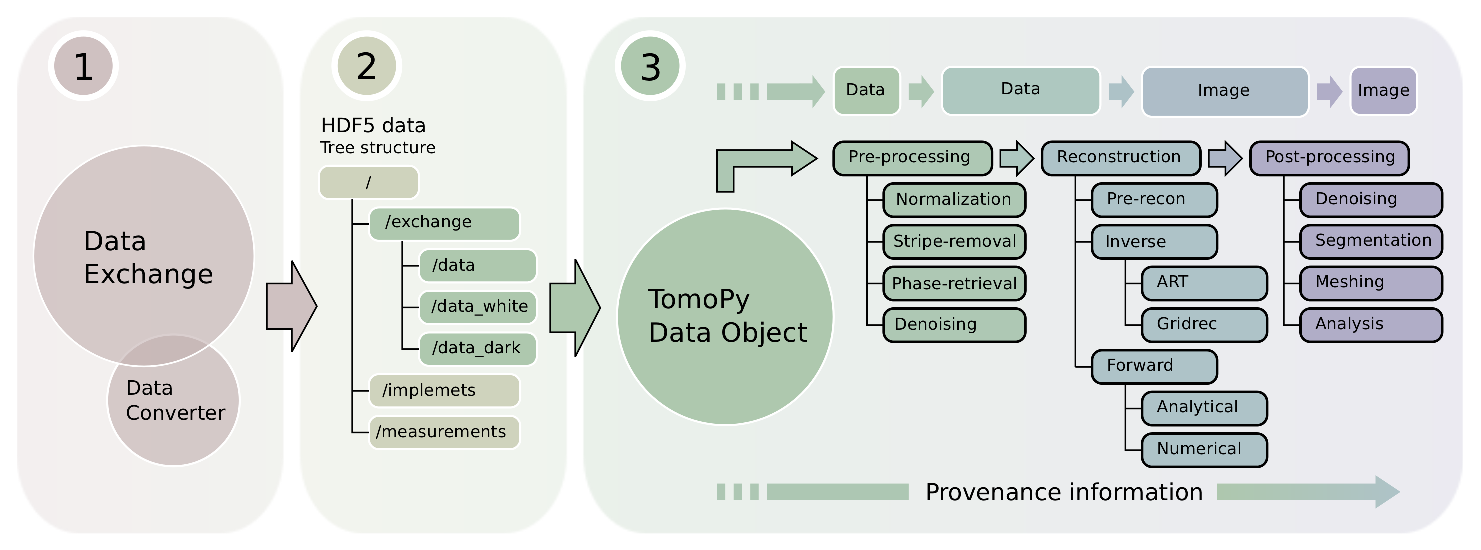
\includegraphics[width=\textwidth]{fig_framework.eps}
\caption{The scotch of the data analysis pipeline.}
\label{fig:ProcessSegmentation}
\end{figure}
\twocolumn


\begin{figure}
\centering
%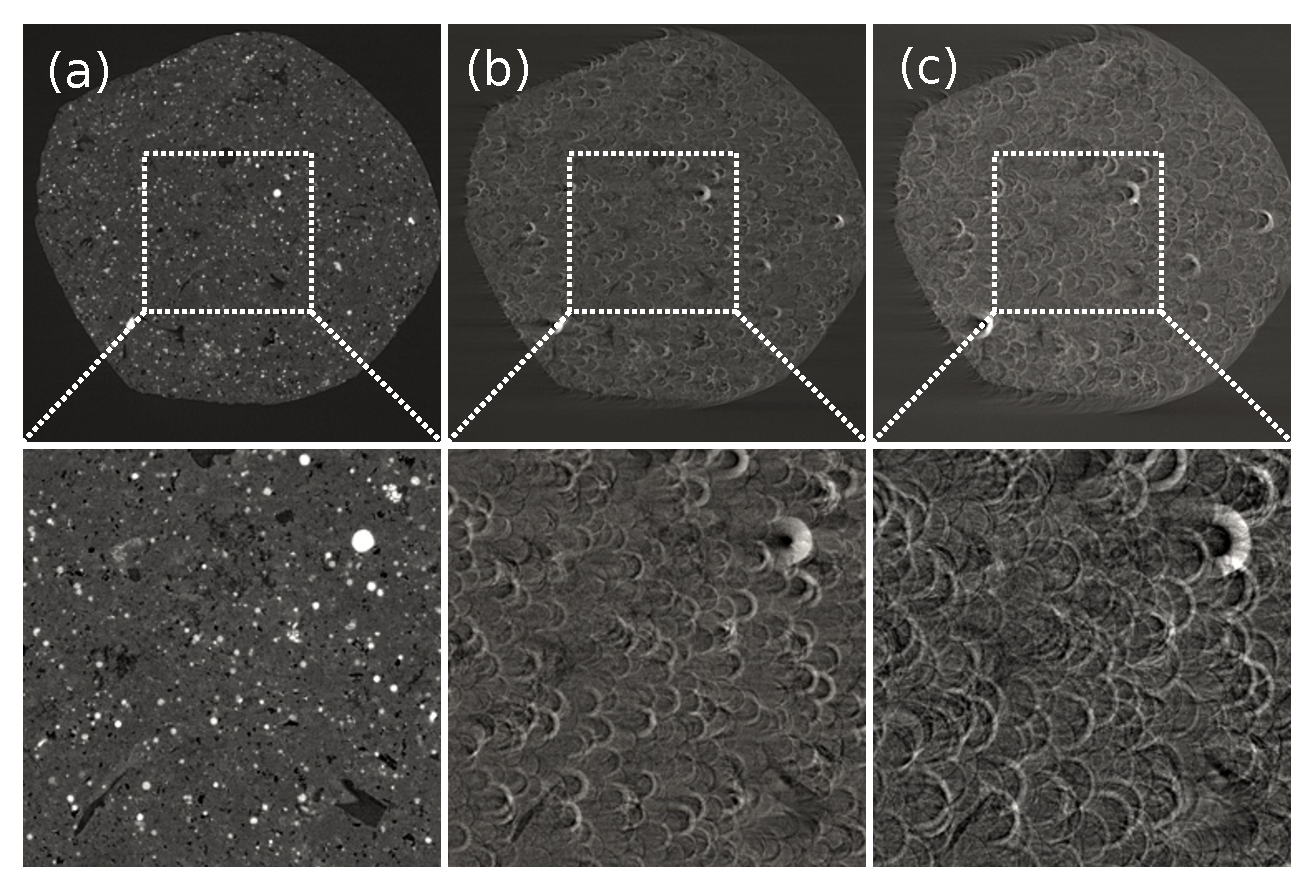
\includegraphics[width=\textwidth]{fig_center1.eps}
\caption{The reconstructed images obtained with different centers of rotations: (a) Correct center, (b) 16 pixels  off-center horizontally, (c) 32 pixels off-center horizontally.}
\label{fig:OptimizeCenter1}
\end{figure}

\begin{figure}
\centering
%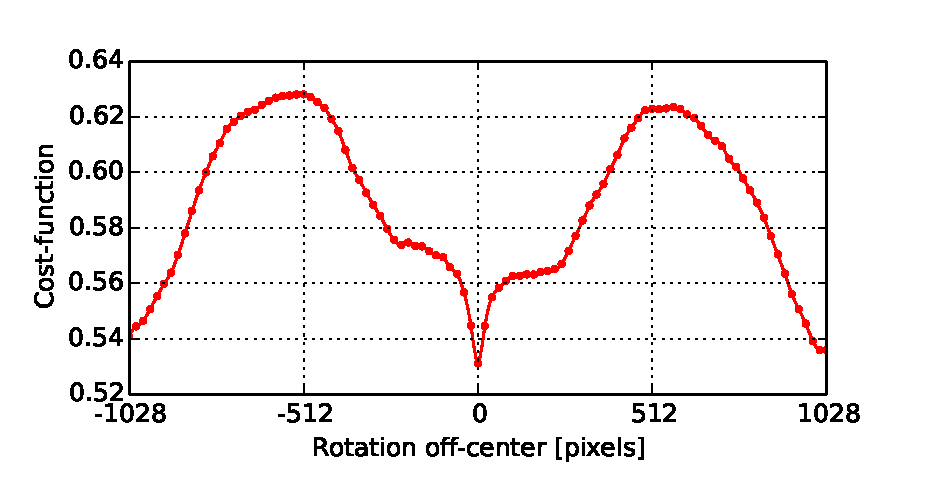
\includegraphics[width=\textwidth]{fig_center2.eps}
\caption{Plot of Shannon entropy as a function of different rotation centers.}
\label{fig:OptimizeCenter2}
\end{figure}


\appendix
\section{Appendix title}

Appendix text.

     % Acknowledgements come after the appendices

\ack{Acknowledgements}

Use of the Advanced Photon Source, an Office of Science User Facility operated for the U.S. Department of Energy (DOE) Office of Science by Argonne National Laboratory, was supported by the U.S. DOE under Contract No. DE-AC02-06CH11357

     % References are at the end of the document, between \begin{references}
     % and \end{references} tags. Each reference is in a \reference entry.

\referencelist[tomopy]

     %-------------------------------------------------------------------------
     % TABLES AND FIGURES SHOULD BE INSERTED AFTER THE MAIN BODY OF THE TEXT
     %-------------------------------------------------------------------------


 

\end{document}                    % DO NOT DELETE THIS LINE
%%%%%%%%%%%%%%%%%%%%%%%%%%%%%%%%%%%%%%%%%%%%%%%%%%%%%%%%%%%%%%%%%%%%%%%%%%%%%%

